% Preambuła
\documentclass[a4paper,10pt]{article}
\usepackage[polish]{babel}
\usepackage[OT4]{fontenc}
\usepackage[utf8]{inputenc}
\usepackage{array}
\usepackage[T1]{fontenc}
\usepackage{hyperref}
\usepackage{caption}
\usepackage{graphicx}

\newcolumntype{R}[1]{>{\raggedleft\arraybackslash}p{#1}}
\newcolumntype{C}[1]{>{\centering\arraybackslash}p{#1}} 
\newcolumntype{L}[1]{>{\raggedright\arraybackslash}p{#1}}

% Część główna

\title{Metody Odkrywania Wiedzy (MOW)\\Projekt analityczny - klasyfikacja\\Dokumentacja wstępna}
\author{Górski Michał\\Napieralski Adam}
\date{13 kwietnia 2020}

\begin{document}
	\maketitle
	
	\section{Cel projektu}
	Celem projektu jest wnikliwa i szeroko zakrojona analiza danych z wykorzystaniem wybranych pakietów i algorytmów zaimplementowanych w środowisku R. Za pomocą dostępnych w R narzędzi stworzone zostaną odpowiednie modele pozwalające na przydzielenie obserwacji do jednej z kategorii na podstawie wartości jej atrybutów. Działania jakie zostaną podjęte przy realizacji zadania projektowego to:
	\begin{itemize}
		\item wstępne przetworzenie/transformacja danych,
		\item podstawowy statystyczny opis danych,
		\item strojenie parametrów algorytmów,
		\item tworzenie i ocena jakości modeli,
		\item opis wyników i przedstawienie wniosków.
	\end{itemize}
 	Celem analizy jest zbudowanie modeli określających typ lasu na postawie pozycji na mapie, nachylenia terenu, typu gleby, odległości od zbiorników wodnych czy dróg.

	\section{Opis danych}
	Dane do projektu pochodzą ze strony UCI Machine Learning Repository \cite{data-source}.
	Zawierają one wstępnie przetworzone dane oparte na surowych danych z 3-osiowego akcelerometru i żyroskopu (opisujących przyspieszenia liniowe i prędkości kątowe) wbudowanych w smartfon.
	Przetworzone zostały przez zastosowanie filtrów i połączenie w próbki - odpowiadające przykładom, dla których wyznaczone zostały wektory 561 atrybutów.\\
	Atrybuty te zawierają m.in. zestawy wartości opisujące: średnią, odchylenie standardowe, średnie odchylenie bezwzględne, wartość największą, wartość najmniejszą, obszar magnitudy sygnału, energię, rozstęp ćwiartkowy, entropię, współczynniki autoregresji, współczynniki korelacji, parametry charakterystyki częstotliwościowej.\\
	Wszystkie te atrybuty są numeryczne, wartości zostały również znormalizowane i ograniczone do przedziału $[-1, 1]$.\\
	Atrybut dyskretny, pełniący rolę interesującego pojęcia domyślnego, to rodzaj wykonywanej aktywności, składający się z kategorii przedstawionych w Tablicy \ref{tab:Klasy1}.
	\begin{center}
	\captionof{table}{Klasy pojęcia domyślnego}
		\begin{tabular}{c | L{4.5cm}} 
			Klasa & Nazwa \\\hline
			1 & Chodzenie \\
	        2 & Wchodzenie po schodach \\
	        3 & Schodzenie \\
	        4 & Siedzenie \\
	        5 & Stanie \\
	        6 & Leżenie \\
	        7 & Siadanie ze stania \\
	        8 & Wstawanie z siedzenia \\
            9 & Położenie z siedzenia \\ 
            10 & Siedzenie z leżenia \\
            11 & Leżenie ze stania \\
            12 & Stanie z leżenia \\
			\hline
		\end{tabular}
		\label{tab:Klasy1}
	\end{center}
	Pełen zbiór zawiera 10 929 przykładów.
	
	\section{Wstępne przygotowanie danych}
	Wszystkie dane, kategoryczne (binarne) oraz nominalne, przedstawione są w postaci liczbowej. W zbiorze nie występują niepełne obserwacje.
	
	Dodane zostaną dwa nowe atrybuty, powstałe poprzez scalenie podobnych istniejących atrybutów. Rodzaje gleby, które są reprezentowane przez wiele atrybutów zostaną zastąpione pojedynczym atrybutem opisującym kategorię gleby. Również atrybuty Wilderness\_Area, zostaną zamienione na jeden atrybut kategoryczny.
	
	Ograniczenie do klas z aktywnościami nieprzejściowymi.
	\begin{center}
		\begin{tabular}{c | L{4.5cm}} 
			Klasa & Nazwa \\\hline
			1 & Chodzenie \\
	        2 & Wchodzenie po schodach \\
	        3 & Schodzenie \\
	        4 & Siedzenie \\
	        5 & Stanie \\
	        6 & Leżenie \\
			\hline
		\end{tabular}
	\end{center}
		
	\section{Wybór i strojenie algorytmów}
		Do analizy wstępnie wybrane zostały algorytmy klasyfikacji:
		\begin{enumerate}
			\item Naiwny Klasyfikator Bayesowski...
% 			(\emph{randomForest}): wymagana parametryzacja drzewa użytego w algorytmie.
			\item SVM - Support Vector Machines (z pakietu \emph{e1071}).\\
			Przy strojeniu sprawdzone zostanie działanie algorytmu dla jądra typu \emph{radial basis} przy różnych wartościach jego parametru $\sigma$. Dodatkowo możliwe jest w mniejszym zakresie sprawdzenie typów jądra \emph{polynomial} czy \emph{sigmoid}.
		\end{enumerate}
		Zależnie od ocenianej na bieżąco sprawności prac, niewykluczona jest klasyfikacja z wykorzystaniem algorytmu lasu losowego \emph{randomForest} i odpowiednia parametryzacja używanego w nim drzewa.\\
		Algorytmy strojone będą z wykorzystaniem oceny pośredniej wyprowadzonej na wybranej z użyciem losowania warstwowego $4/5$ części zbioru pełnego. Stosowana będzie tam \emph{k}-krotna walidacja krzyżowa (\emph{k}-CV) z $k=5$ (Rys. \ref{fig:podzial}).
		
		Dodatkowe szczegóły dotyczące wyboru algorytmu i dokładnego określenia parametrów podjęte zostaną na etapie realizacji analizy, uzależniając ją od stopnia skomplikowania zadania projektowego.
		
    \begin{figure}[h]
        \centering
        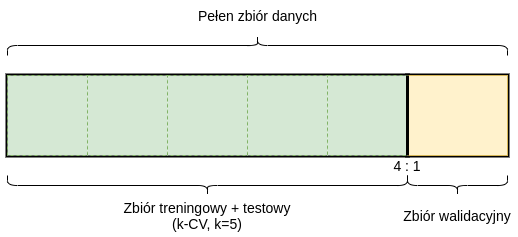
\includegraphics[width=0.8\textwidth]{Podzial_zbioru.png}
        \caption{Podział zbioru danych na podzbiory.}
        \label{fig:podzial}
    \end{figure}
    
 	\section{Ocena jakości modeli}
 	Prowadzenie oceny pośredniej nastąpi za pomocą wspomnianej procedury k-krotnej walidacji krzyżowej (\emph{k}-CV). Ocena końcowa wyprowadzona zostanie zgodnie z procedurą \emph{holdout} na nieużywanej wcześniej części zbioru danych.
 	Do oceny uwzględnione zostaną rozkłady pomyłek, wyznaczona zostanie macierz pomyłek na zbiorze oraz powiązane z nią współczynniki. Na ich podstawie możliwe będzie wykreślenie krzywej ROC oraz wyznaczenie AUC.
 		
 		
\begin{thebibliography}{9}
\bibitem{data-source}
Smartphone-Based Recognition of Human Activities and Postural Transitions Data Set 
\url{http://archive.ics.uci.edu/ml/datasets/Smartphone-Based+Recognition+of+Human+Activities+and+Postural+Transitions}

\end{thebibliography}
\end{document}
